\documentclass[aps, prc, reprint, amsmath, groupedaddress, nofootinbib]{revtex4-1}
\usepackage[compat=1.1.0]{tikz-feynman}
\usepackage[utf8]{inputenc}
\usepackage{hyperref}
\usepackage{amsmath}
\usepackage{amssymb}
\usepackage{amsfonts}
\usepackage{tabularx}
\usepackage{booktabs}
\usepackage{graphicx}
\usepackage{color}
\usepackage{multirow}
\usepackage[inline]{enumitem}
\graphicspath{{fig/}}
\definecolor{theblue}{RGB}{0,50,230}
\usepackage{appendix}
\hypersetup{
  colorlinks=true,
  linkcolor=theblue,
  citecolor=theblue,
  urlcolor=theblue
}



\newcommand{\trento}{T\raisebox{-0.5ex}{R}ENTo}
\newcommand{\nch}{N_\text{ch}}
\newcommand{\sqrts}{\sqrt{s_{NN}}}
\newcommand{\T}{\tilde{T}}
\newcommand{\paddedhline}{\noalign{\smallskip}\hline\noalign{\smallskip}}
\newcommand{\dnchdy}{dN_\text{ch}/d\eta}
\newcommand{\dndypP}{dN_\text{pPb}/d\eta}
\newcommand{\dndyPP}{dN_\text{PbPb}/d\eta}
\newcommand{\x}{\mathbf x}
\newcommand{\y}{\mathbf y}
\newcommand{\z}{\mathbf z}
\newcommand{\trans}{^\intercal}

\newcommand{\Raa}{R_{AA}}
\newcommand{\vv}{v_2\{2\}}
\newcommand{\vvv}{v_3\{2\}}
\newcommand{\vnv}{v_n\{2\}}
\newcommand{\ppi}{\frac{\partial}{\partial p_i}}
\newcommand{\ppj}{\frac{\partial}{\partial p_j}}
\newcommand{\ppl}{\frac{\partial}{\partial p_l}}
\newcommand{\Kpara}{\kappa_{\|}}
\newcommand{\Kperp}{\kappa_{\perp}}
\newcommand{\Ppara}{\hat{P}^{\|}}
\newcommand{\Pperp}{\hat{P}^{\perp}}

\begin{abstract}
Current observation of open charm in heavy-ion collisions shows unexpectedly large momentum anisotropy and small nuclear modification factor, posing a challenge to the theoretical understanding of the nature of coupling between heavy quark and the medium.
Linear Boltzmann transport and Langevin diffusion are two popular kinetic models for heavy quark in-medium propagation.
In this work, we develop a hybrid heavy quark transport model that combines the strengths of both: 
heavy quarks are evolved with Langevin diffusion using an empirical diffusion constant and scattering processes treated linear Boltzmann equations with perturbative matrix elements.
The Langevin component is a complementary contribution to the linear Boltzmann equation when perturbative scattering is inadequate.
Both elastic and inelastic scatterings are included in the Boltzmann component.
The Landau-Pomeranchuk-Migdal effect is treated effectively via gluon formation time and detailed balance is imposed between gluon emission and absorption.
With the hybrid model, we study the heavy flavor momentum anisotropic, nuclear modification factor, and correlation observables in A-A collisions at the RHIC and the LHC energies.
Comparing to available D and B meson data, we constrain the diffusion constant of the Langevin component.

\end{abstract}


\begin{document}


\title{A hybrid heavy quark transport model in a quark-gluon plasma that couples linear Boltzmann equation and Langevin diffusion dynamics}
\author{Weiyao Ke}
\author{Yingru Xu}
\author{Steffen A.\ Bass}
\affiliation{Department of Physics, Duke University, Durham, NC 27708-0305}
\date{\today}
\maketitle

\section{Introduction}
Heavy flavors are an ideal probe of the properties of the strongly coupled  quark-gluon plasma produced in relativistic heavy-ion collisions.
Due to their large mass compared to the temperature scale achieved in the experiments \cite{}, thermal production of heavy quarks from medium is highly suppressed; therefore the dominant source of heavy flavors are initial hard production vertex.
Produced at early times of the collision, these flavor tagged probes experience the full time evolution of the quark-gluon plasma and their numbers is almost conserved.
The mass effect sets an additional scale to the problem and brings rich physics to the heavy flavor sector.
In the high transverse momentum region, heavy quarks can lose energy perturbatively and merge into the regime of jet energy loss study;
in the low momentum region, the mass effect $M\gg T$ delays the heavy quark thermalization time, providing a window to study the non-equilibrium dynamics of QCD.
Therefore the study of heavy flavor observables is a unique way to understand the dynamics of the quark-gluon plasma and the heavy quark in-medium propagation itself.


\section{Understanding heavy quark propagation with a hybrid transport}
Open flavor heavy quarks are flavor tagged probes with large masses compared to the typical energy scale of the medium produced in relativistic heavy-ion collisions ($M \gg T$).
This enables one to treat heavy quarks as good quasi-participles and dilute in the medium.
For the study of open flavor we neglect the back reaction from heavy quark to the medium. 
In this approximation, the main features of heavy-flavor-medium interactions are captured in a linearized Boltzmann equation.
\begin{eqnarray}
  \frac{\partial}{\partial t}f_Q - \frac{\vec{p_1}}{E_1}\cdot\nabla f_Q  = 
\mathcal{C}[f_Q]
%C_i^{2\rightleftharpoons 2}[f_Q] + C_i^{2\rightleftharpoons 3}[f_Q]
\end{eqnarray}
The collision processes with medium particles change the heavy quarks' distribution function $f_Q(t, \vec{x}, \vec{p})$.

The precise knowledge of the collision integral on the right is hard to obtain.
In principal, these processes should be calculable from the fundamental theory using perturbative-QCD. 
However, analyzing in-medium processes are much more complex than in vaccum even at leading order. 
Also, the temperatures reached in current experiments are not high enough, which brings large ambiguity in the calculation through the scale dependence of the QCD coupling constant.
Finally, a practical leading order pQCD cross-sections usually involves a relative large multiplicative $K$-factor to describe data.
A different perspective of analyzing the collision integral starts with the assumption that medium kicks to heavy quark propagation are frequent and soft.
This assumption reduces the linear Boltzmann equation to a Fokker-Plank equation where heavy quark undergoes diffusion dynamics. 
The diffusion approximation has the advantage that the complex underlying dynamics are represented by a few transport coefficients--drag and diffusion. 
It is easier to extract these numbers from empirical data than ab initio evaluation. 
The drawbacks are it only works when interactions are indeed soft and frequent and the relation between the obtained empirical transport coefficients to the fundamental theory is hard to establish.

In this paper, we would like to take advantages from both perspectives.
We divided the collision term in the linear-Boltzmann equation into two parts.
Part one--the scattering component--contains scattering processes that what we can calculate start from the fundamental theory.
Part two--the diffusion component--solves diffusion dynamics with empirical transport coefficients that parametrize what is missing in part one to describe the data. 
To avoid confusion, we shall call them residue transport coefficients in the sense that it contains interactions or corrections not included in part one.
We have noticed that such a separation of matrix-element scattering and diffusion has been proposed for the study of jet propagation.
The separation in \cite{} is based on momentum transfer and applied order-by-order to perturbative-QCD calculation of jet-medium interaction.
In our study, we don't restrict the content of the residue transport coefficients to be of pQCD origin.
In this way, our model build upon existing knowledge of the scattering matrix-element from pQCD and can be systematically improve the residue transport coefficient to describe the experiments while only varying parameter in pQCD within a reasonable range.

\subsection{Part one, scattering dynamics}
At lowest order in the coupling constant, heavy quarks can scattering elastically with a light quark (anti-quark) or a gluon f, as shown in Fig. \ref{plots:feyn-elastic}.
We will keep use the term ``elastic" and later ``inelastic" to distinguish particle number conserving and particle number changing processes and their associated energy loss.
For quark-gluon scattering, there are three diagrams corresponds to $s, t,$ and $u$ channel exchange; only $t$ channel contributes to quark-quark scattering.
The matrix-elements for these processes are calculated at leading order pQCD (see \ref{appendix:matrix-element}).
The $t$ channel gluon exchange in the vacuum causes divergence in cross-section as the momentum transfer vanishes,
\begin{eqnarray}
d\sigma \propto \frac{1}{t^2} dt,
\end{eqnarray}
but inside a quark-gluon plasma, those soft gluon exchange is screened by the surrounding color charges and the propagator is replaced by a hard-thermal loop propagator \cite{}.
Here, we simply uses the leading order Debye mass as a regulator, $t \rightarrow t - m_D^2$.

At high energy, inelastic processes which involves gluon radiation in the final state shown in Fig. \ref{plots:feyn-inelastic} becomes important.
Although the inelastic processes seem to be one order higher in the coupling conspropagtion of the tant than the elastic processes, due to the divergence of the almost on-shell intermediate propagator, its contribution to energy loss increases with incident heavy quark energy and eventually dominates over elastic energy loss \cite{}.
Boltzmann equation with only the gluon radiation radiation violates detail balance, and the theory won't have a correct thermal solution.
To solve this issue, we include the reverse process of radiation, namely the gluon absorption process.
The matrix-element for the absorption relates to the radiation matrix-element by bending the final state gluon emission line to the initial state ($k^\mu \rightarrow -k^\mu$).
An additional gluon in the initial state brings an additional Boltzmann factor $e^{-k/T}$, so we expect it to be less important at high energy (low temperature) but essential for heavy quark thermalization.
We shall study numerically that under what conditions that the inclusion of the gluon absorption process is important to energy loss.

A complication for inelastic processes is that the radiated gluon takes finite amount of time to be fully resolved from the source. 
Within the formation time, the effects of multiple soft collisions add up  coherently in a destructive way to suppress the gluon radiation, know as the Landau-Pomeranchuk-Migdal (LPM) effect \cite{}.
With LPM effect, emission of a single gluon dependents on multiple collisions experienced by the heavy quark, but this is difficult to implement in a Boltzmann equation setup where scatterings are localized in space-time.
In our model, we mimic the LPM effect by considering the physical interpretation of the gluon formation time $\tau_f$,
\begin{eqnarray}
\tau_f &=& \frac{2(1-x)k}{k_\perp^2 + x^2M^2} \\
x &=& \frac{k^+}{E^+}
\end{eqnarray}
A gluon cannot be fully resolved from the heavy quark shorter than time scale, therefore we restrict the phase space integral of the emitted gluon   by a coherence factor,
\begin{eqnarray}
d\Gamma_k \rightarrow \left(1 - \cos\left(\Delta t/\tau_f\right) \right)d\Gamma_k,
\end{eqnarray}
where $\Delta t$ is the time elapsed from the last radiation.
In the infinite time limit $\Delta t \rightarrow \infty$, the average of the coherence factor goes to $1$; while with finite $\Delta t$, the radiation of gluon that has not fully formed yet (i.e. $\tau_f > \Delta t$) is suppressed.
With this prescription, the evolution of a heavy quark becomes history dependent. 
It is not trivial to tell if the Boltzmann equation modified in this way should thermalize as $t\rightarrow \infty$, so we tested in actually simulations and confirm the model approaches correct thermal limit.

\begin{figure}
\feynmandiagram [xscale=.95, yscale=1, horizontal=a to b] {
  p1 -- [fermion] a--b[fermion] -- [fermion] p3 ,
  p2 -- [gluon] a,
  p4 -- [gluon] b,
};
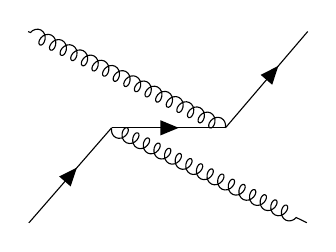
\begin{tikzpicture}[xscale=.95, yscale=1.]
  \begin{feynman}
    \diagram [horizontal=a to b] {
      i1 %[particle=\(Q\)]
      -- [fermion] a
      -- [draw=none] f1,% [particle=\(g\)],
      a -- [fermion] b,
      i2 %[particle=\(Q\)]
      -- [anti fermion] b
      -- [draw=none] f2,% [particle=\(g\)],
    };
    \diagram* {
      (a) -- [gluon] (f2),
      (b) -- [gluon] (f1),
    };
  \end{feynman}
\end{tikzpicture}
\feynmandiagram [xscale=1.2, yscale=.8, horizontal=p2 to p4] {
  p2 [particle=$g$]-- [gluon] b -- [gluon] p4 [particle=$g$],
  a -- [gluon] b,
  p1 [particle=$Q$] -- [fermion] a -- [fermion] p3 [particle=$Q$],
};
\feynmandiagram [xscale=1.2, yscale=.8, horizontal=p1 to p3] {
  p2 [particle=$q$] -- [fermion, edge label=$p_2$] a -- [fermion, edge label=$p_4$] p4 [particle=$q$],
  a -- [gluon, momentum=$q$] b,
  p1 [particle=$Q$] -- [fermion, edge label=$p_1$] b -- [fermion, edge label=$p_3$] p3 [particle=$Q$],
};
\caption{Elastic processes. The first three diagrams contribute to heavy quark (Q) - gluon (g) scattering, the last one contributes to a light (anti-)quark (q) scattering. Intermediate propagators are screened by a Debye mass in case of soft divergence.}\label{plots:feyn-elastic}
\end{figure}

Given this scattering processes, the linear Boltzmann equation is solved by transport and an ensemble of heavy quark according to the collision rates of different reaction channels.
The collision rates for elastic scatterings, gluon radiation and gluon absorption are,
\begin{eqnarray}
    R_{22,i} &=& \frac{d_i/\nu_i!}{2E_1} \int d \Gamma_{p_3,p_4}^{p_2}(p_1) f_i(p_2)  \overline{|M_{22}|^2},
   \nonumber
  \\
  R_{23,i} &=& \frac{d_i/\nu_i!}{2E_1} \int d \Gamma_{p_3,p_4,k}^{p_2}(p_1) f_i(p_2) 
\overline{|M_{23}|^2},
  	 \nonumber
  \\
  R_{32,i} &=& \frac{d_i/\nu_i!}{2E_1} \int d \Gamma_{p_3,p_4}^{p_2,k}(p_1) f_i(p_2)f_g(k)
\overline{|M_{32}|^2}.
  	 \nonumber
\end{eqnarray}
Where the N-body phase-space integration,
\begin{eqnarray}
\nonumber
d\Gamma_{\{\textrm{out}\}}^{\{\textrm{in}\}}(p_1) = \prod_{\{\textrm{in, out}\}} \frac{dp_i^3}{2E_i(2\pi)^3} (2\pi)^4\delta^4(p_1+P_{\text{in}} - P_{\textrm{out}})
\end{eqnarray}
$d_i$ counts the degeneracy of the incoming medium particle and $\nu_i$ counts the number of identical gluons in the initial / final state of the collision.
The medium partons are assumed and reached thermal equilibrium with a Maxwell distribution function, 
\begin{eqnarray}
f(p,x) = \exp\left(-\frac{p \cdot u(x)}{T(x)}\right).
\end{eqnarray}
The space-time temperature $T$ and velocity $u$ profiles are obtained from the 2+1D viscous relativistic hydrodynamic calculations \cite.

\begin{figure}
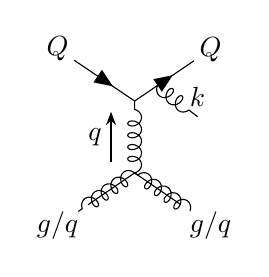
\begin{tikzpicture}
  \begin{feynman}
    \diagram [xscale=0.8, yscale=.6, vertical=a to b] {     
      i2 [particle=\(g/q\)]
        -- [gluon] b
        -- [gluon] f2 [particle=\(g/q\)]],
      b -- [gluon, momentum=$q$] a,
      i1 [particle=\(Q\)]
        -- [fermion] a
        -- [fermion] f1 [particle=\(Q\)],
    };
    \vertex [below right=.2 cm and .8 cm of a, label=\(k\)] (r);
    \draw [gluon] ($(a)!0.3!(f1)$) -- (r);
    \draw  (i2)--(b);
     \draw  (b)--(f2);
  \end{feynman}
\end{tikzpicture}
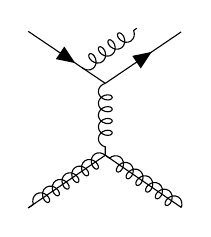
\begin{tikzpicture}
  \begin{feynman}
    \diagram [xscale=0.8, yscale=0.6, vertical=a to b] {     
      i2  -- [gluon] b
        -- [gluon] f2,
      a -- [gluon] b,
      i1 -- [fermion] a
        -- [fermion] f1,
    };
    \vertex [above right=.7 cm and .4 cm of a] (r);
    \draw [gluon] ($(i1)!0.7!(a)$) -- (r);
    \draw  (i2)--(b);
     \draw  (b)--(f2);
  \end{feynman}
\end{tikzpicture}
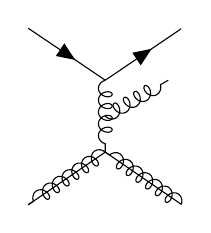
\begin{tikzpicture}
  \begin{feynman}
    \diagram [xscale=0.8, yscale=.6, vertical=a to b] {     
      i2 %[particle=\(g\)]
        -- [gluon] b
        -- [gluon] f2, %[particle=\(g\)]],
      a -- [gluon] b,
      i1 %[particle=\(Q\)]
        -- [fermion] a
        -- [fermion] f1, %[particle=\(Q\)],
    };
    \vertex [below right=.0 cm and .8 cm of a] (r);
    \draw [gluon] ($(a)!0.5!(b)$) -- (r);
    \draw  (i2)--(b);
     \draw  (b)--(f2);
  \end{feynman}
\end{tikzpicture}
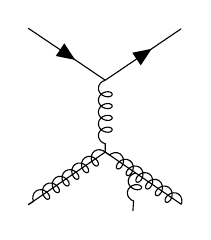
\begin{tikzpicture}
  \begin{feynman}
    \diagram [xscale=0.8, yscale=.6, vertical=a to b] {     
      i2 %[particle=\(g\)]
        -- [gluon] b
        -- [gluon] f2, %[particle=\(g\)]],
      a -- [gluon] b,
      i1 %[particle=\(Q\)]
        -- [fermion] a
        -- [fermion] f1, %[particle=\(Q\)],
    };
    \vertex [below right=.75 cm and .35 cm of b] (r);
    \draw [gluon] ($(i2)!0.6!(b)$) -- (r);
    \draw  (i2)--(b);
     \draw  (b)--(f2);
  \end{feynman}
\end{tikzpicture}
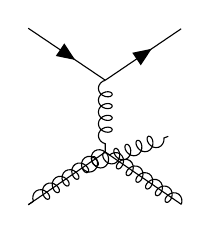
\begin{tikzpicture}
  \begin{feynman}
    \diagram [xscale=0.8, yscale=.6, vertical=a to b] {     
      i2 %[particle=\(g\)]
        -- [gluon] b
        -- [gluon] f2, %[particle=\(g\)]],
      a -- [gluon] b,
      i1 %[particle=\(Q\)]
        -- [fermion] a
        -- [fermion] f1, %[particle=\(Q\)],
    };
    \vertex [above right=.2 cm and .8 cm of b] (r);
    \draw [gluon] ($(b)!0.3!(f2)$) -- (r);
    \draw  (i2)--(b);
     \draw  (b)--(f2);
  \end{feynman}
\end{tikzpicture}
\caption{Inelastic process. Heavy quark collide with a meidum light (anti-)quark or gluon and radiates an additional gluon.}\label{plots:feyn-inelastic}
\end{figure}

Finally for the coupling constant in these matrix-elements, we utilize the leading order running coupling constant with three flavors of quark \cite{},
\begin{eqnarray}
\alpha_s(\mu^2) = \frac{4\pi}{9}
\begin{cases}
1/\ln\left(-\mu^2/\Lambda^2\right),\hfill \mu^2 < 0 \\ 
\frac{1}{2} - \frac{1}{\pi}\arctan\left[\frac{\ln\left(\mu^2/\Lambda^2\right)}{\pi}\right],\mu^2 > 0
\end{cases}
\end{eqnarray}
The QCD scale is set at $\Lambda = 200$~MeV.
For elastic scattering, we evaluate $\alpha_s$ at the typical momentum transfer of the process. For the gluon emission / absorption vertex in inelastic scatterings, we choose $\alpha_s(k_\perp^2)$ \cite{}.
Inside a medium, there is an additional scale defined by the temperature $T$, we use it as a lowest cutoff for the energy scale of the process,
\begin{eqnarray}
\alpha_s(Q^2) \rightarrow \alpha_s(\max\{Q,\nu T\})
\end{eqnarray}
$\nu$ the only parameter we will tune in the scattering component of the model.

\subsection{Part two, diffusion dynamics}
The diffusion dynamics of the heavy quark is simulated by solving Langevin equations in the Ito-discretization scheme,
\begin{eqnarray}
\Delta \vec{x}_i &=& \frac{\vec{p}_i}{E} \Delta t	\\
\Delta \vec{p}_i &=& -\Gamma \vec{p}_i \Delta t + \Delta t \vec{\xi}
\end{eqnarray}
The momentum change comes from a drag term with a momentum drag coefficient $\Gamma$ and a thermal random force $\vec{\xi}$. 
The random force has zero mean and covariance structure:
\begin{eqnarray}
\langle \xi_i \xi_j \rangle = \frac{1}{\Delta t}\left(\Kpara \frac{p_i p_j}{p^2} + \Kperp \left(\delta_{ij} - \frac{p_i p_j}{p^2}\right) \right)
\end{eqnarray}
In this study, we assume the residue momentum diffusion is isotropic $\Kpara=\Kperp=\kappa$.
The drag $\Gamma$ and the momentum diffusion coefficient $\kappa$ need to satisfy the Einstein relation to guarantee the correct thermal limit is reached as time approaches infinity,
\begin{eqnarray}
\Gamma &=& \frac{\kappa}{2TE} - \frac{d\kappa}{dp^2}
\end{eqnarray}
We choose momentum diffusion $\kappa$ as the independent variable in our parametrization.
If temperature is the only scale in the problem, we expect $\kappa$ to scale as $T^3$.
Additional, we consider the possibility of non-perturbative contribution to the residue transport, which only happens at low energy and low temperature and arrived at this simple ansatz,
\begin{eqnarray}
\frac{\kappa}{T^3} = \left(A + \frac{B}{ET}\right)
\end{eqnarray}

\section{Tests in a static medium}
\subsection{Thermalization}
\begin{figure}
\includegraphics[width=\columnwidth]{charm-plot/thermalization.pdf}
\caption{The approach to thermalization of the linear Boltzmann equation with elastic processes only (red dot), elastic with radiation processes (green dashed), and elastic with both radaition and absorption processes (blue solid). The static medium has a temperature $T = 0.4$ GeV. $10^4$ heavy quarks are initialized with $E = 10$ GeV at $t = 0$.}\label{plots:thermalization}
\end{figure}
We first show our implementation of the above model gives the correct thermal limit. 
The quantify the approach to equilibrium of an ensemble of heavy quarks in side a static medium with a fixed temperature $T_0$, we define the following quantity,
\begin{eqnarray}
\Delta S = \frac{1}{N}\sum_i \ln f_0(E_i) - \int f_0(p)\ln f_0(p) dp^3
\end{eqnarray}
$f_0 \propto \exp(-E/T)$ is the relativistic Boltzmann distribution function at temperature $T$. 
The second term is the entropy at that temperature, while the first term is the ensemble average of one-particle entropy at that temperature.
This difference $\Delta S$ defines a ``distance" towards the equilibrium state, and vanishes when the thermal equilibrium is reached.
If the ensemble is not far from thermal equilibrium and can be characterized by an effective temperature $T_{\textrm{eff}}$ that the distribution function $f(E)\sim \exp(-E/T_{\textrm{eff}})$, then
\begin{eqnarray}
\nonumber
\Delta S &\sim& \frac{1}{T}\int  e^{-E/T_{\textrm{eff}}} E dp^3 - \frac{1}{T}\int e^{-E/T} E dp^3 \\
&=& \frac{T_\textrm{eff}-T}{T}
\end{eqnarray}
is an estimate of the deviation of the effective temperature from the temperature of the thermal bath.
Figure \ref{plots:thermalization} shows the time-evolution of $Delta S$ of heavy quarks inside thermal bath $T=0.4$ GeV with initial energy $E_0 = 10$ GeV.
With elastic process only, the system thermalize after about $150$ fm/$c$.
If we further turn on radiation process, the equilibrium is reached in a shorter amount of time, but it is wrong equilibrium.
The effective temperature is lower than the temperature of the thermal bath.
This is the consequence from breaking detailed balance with radiation process only.
By adding the absorption processes, the correct equilibrium is reached.
We also point out that the inclusion of absorption processes only start to make difference when the system is not far from equilibrium.

\subsection{Collision rates and Energy loss}
We can integrate collision rates using Equations \ref{•}, and calculate energy loss of a heavy quark by inserting $\Delta E$ into the integration of differential rates.
This is straight forward for elastic processes, but since the rates of inelastic processes depend on collision history, a meaningful rate and energy loss in side a medium can only be obtained by an actually Monte Carlo simulation.
Moreover, this history dependence is the reason that our rates and energy loss is not only a function of the incident energy ($E$) and medium temperature ($T$) but also the medium size (path length $L$).

\begin{figure*}
\includegraphics[width=\textwidth]{BoxRate.pdf}
\caption{}\label{plots:BoxRate}
\end{figure*}

In Figure \ref{plots:dE-E}, we plot energy loss fraction $\Delta E/E$ for elastic process (first row) and inelastic process (second row) as function of $E$ for different path length and temperature.
The elastic energy loss fraction increases as temperature and decreases for large energy.
At low energy, the heavy quark starts to gain net energy from the medium as which manifests as $\Delta E < 0$.
For the case of inelastic energy loss, we study the effect of gluon absorption process by comparing $\Delta E/E$ with radiation process only and with both radiation and absorption processes.
We find that gluon absorption process does not affect the energy loss at low temperature or high energy heavy quark as expected.
For high temperature such as $T=0.6$ GeV and energy below $10$ GeV, the gluon absorption process makes a notable difference.
Radiation process always leads to a positive average energy loss, but with absorption process, heavy quarks with very low energy actually on average gain energy from the medium.

In Figure \ref{plots:dE-L}, we show the path length dependence of the two energy loss mechanism.
Here, we plot the energy loss fraction per unit length, with length measured in units of inverse temperature.
The key observation is that elastic energy loss per unit length is a constant while for inelastic energy loss, this quantity first increases from zero for small path length and then gradually approaching a limit for large path length, showing a different medium size dependence of energy loss from the elastic process.
The non-linear path length dependence $\Delta E \propto L^2$ is actually a characteristic behavior of the coherence effect in a finite length medium \cite{}. 
In our effective implementation of LPM, this behavior arises because gluon radiation with
\begin{eqnarray}
\tau_f \ll L.
\end{eqnarray}
is suppressed, and therefore the inelastic energy loss for a thin medium is very small.
As $L$ increases, a high energy heavy quark could have radiated gluons with formation time $\tau_f$ multiples times $N \propto L/\tau_f$ where each radiation carries off a typical amount of energy. 
As a result the energy loss grows again linearly with path length.


\begin{figure*}
\includegraphics[width=\textwidth]{E_Eloss.pdf}
\caption{}\label{plots:dE-E}
\end{figure*}

\begin{figure*}
\includegraphics[width=\textwidth]{L_Eloss.pdf}
\caption{}\label{plots:dE-L}
\end{figure*}

\subsection{$R_{AA}$ in a static medium}
\begin{figure}
\includegraphics[width=\columnwidth]{Box_Raa.pdf}
\end{figure}

\subsection{$R_{AA}$ in a static medium}
Finally, for our study in a static medium, we calculate the $R_{AA}$ of charm and bottom quark in a medium $T=0.4$ GeV of size $L=4$ fm.

\section{Calibration of the model at LHC using Bayesian analysis}


\begin{appendices}
\section{Matrix elements}
\label{appendix:matrix-element}
\begin{widetext}
\begin{eqnarray}
\overline{|M_{Q+q\rightarrow Q+q}|^2} &=& \frac{64\pi^2}{9}\alpha_s^2 \frac{(u-M^2)^2 + (s-M^2)^2 + 2 M^2 t}{(t-m_D^2)^2}
\end{eqnarray}
\begin{eqnarray}
\overline{|M_{Q+g\rightarrow Q+g}|^2} &=& \pi^2 \left\{
32\alpha_s^2 \frac{(s-M^2)(-u+M^2)}{(t-m_D^2)^2} \right. \\ \nonumber
&+&\frac{64}{9}\alpha_s^2 \frac{(s-M^2)(-u+M^2)+2M*2(s-M^2) + 4M^4}{(s-M^2+m_D^2)^2} \\ \nonumber
&+&\frac{64}{9}\alpha_s^2 \frac{(s-M^2)(-u+M^2)+2M*2(u-M^2) + 4M^4}{(-u+M^2+m_D^2)^2} \\ \nonumber
&+&\frac{16}{9}\alpha_s^2 \frac{M^2(4M^2 - t)}{(-u+M^2+m_D^2)(s-M^2+m_D^2)} \\ \nonumber
&+& 16 \alpha_s^2 \frac{(s-M^2)(-u+M^2)+M^2(s-u)}{(t-m_D^2)(s-M^2+m_D^2)} \\ \nonumber
&-& \left. 16 \alpha_s^2 \frac{(s-M^2)(-u+M^2)-M^2(s-u)}{(t-m_D^2)(-u+M^2+m_D^2)}\right\} \\
\overline{|M_{Q+q\rightarrow Q+q+g}|^2} &=& \overline{|M_{Q+q\rightarrow Q+q}|^2} 48 \pi \alpha_s (1-\bar{x})^2 \left(\frac{\vec{k}_\perp}{k_\perp^2 + x^2 M^2} 
+ \frac{\vec{q}_\perp - \vec{k}_\perp}{(\vec{q}_\perp-\vec{k}_\perp)^2 + x^2 M^2 + m_D^2}
\right)^2 
\end{eqnarray}
\begin{eqnarray}
\overline{|M_{Q+g\rightarrow Q+g+g}|^2} &=& \overline{|M_{Q+g\rightarrow Q+g, \textrm{t-channel}}|^2} 48 \pi \alpha_s (1-\bar{x})^2 \left(\frac{\vec{k}_\perp}{k_\perp^2 + x^2 M^2} 
+ \frac{\vec{q}_\perp - \vec{k}_\perp}{(\vec{q}_\perp-\vec{k}_\perp)^2 + x^2 M^2 + m_D^2}
\right)^2 
\end{eqnarray}
\end{widetext}

\section{Evolution with both scattering and diffusion dynamics}
With a transport $\hat{T} = -v\cdot \partial_x$, a scattering $\hat{C}$, and a diffusion $\hat{D}$ operator in the hybrid transport equation,
\begin{eqnarray}
\frac{\partial f}{\partial t} = \left( \hat{T} + \hat{C} + \hat{D} \right) f
\end{eqnarray}
The formal solution is,
\begin{eqnarray}
f_{\Delta t} = e^{\int_0^{\Delta t}  \left( \hat{T} + \hat{C} + \hat{D} \right) dt}f_0
\end{eqnarray}
Assume the time variance of the medium are slow and decompose the joint operation into separate operations.
\begin{eqnarray}
e^{ \Delta t\left(\hat{T} +\hat{C} + \hat{D} \right)} &=&
\nonumber
e^{\Delta t \left(\hat{T} + \hat{D}\right) } e^{\Delta t \hat{C}}   e^{-\frac{\Delta t^2}{2} [\hat{T}+\hat{D}, \hat{C}]}\left(1+O(\Delta t^3)\right) \\
\nonumber
&=& \frac{1}{2}  \left\{
1+\Delta t \left( \hat{T}+\hat{D} \right), 1+\Delta t C
\right\} + O(\Delta t^3) 
\end{eqnarray}
The operator $1 + \Delta t ( \hat{T}  + \hat{D} )$ stands for a ``Diffusion" step in the simulation; the operator $1+\Delta t \hat{C}$ stands for a ``Scattering" step in the simulation. 
Therefore, we design the following simulation procedure.
\begin{itemize}
\item For each step, choose a $\Delta t$ in lab frame small enough that total scattering probability $P_c \ll 1$.
\item Determine the ordering of diffusion step and scattering step with 50-50\% chance
\item If diffusion operates before scattering.
\begin{itemize}
\item[Step 1.] $(t, x, p) \xrightarrow{\textrm{Diffusion}} (t+\Delta t, x', p^*)$.
\item[Step 2.] $(t+\Delta t, x', p^*) \xrightarrow{\textrm{Scattering}} (t+\Delta t, x', p')$.
\end{itemize}
\item If diffusion operates after scattering.
\begin{itemize}
\item[Step 1.] $(t, x, p) \xrightarrow{\textrm{Scattering}} (t, x, p^*)$.
\item[Step 2.] $(t, x, p^*)  \xrightarrow{\textrm{Diffusion}} (t+\Delta t, x', p')$.
\end{itemize}
\end{itemize}

\section{Calculation of $v_n\{2\}$ and $v_2\{EP\}$}
Cumulant method correlates a heavy meson with a light particle to estimate $v_n$.
\begin{eqnarray}
v_n\{2\} &=& \frac{d_n\{2\}}{\sqrt{c_n\{2\}} } \\
d_n\{2\} &=& \left\langle \frac{\Re\{pQ^*\}}{mM} \right\rangle_{w = mM} \\
c_n\{2\} &=& \left\langle \frac{|Q|^2-M}{M(M-1)} \right\rangle_{w = M(M-1)}
\end{eqnarray}
\end{appendices}
\end{document}